%% ========================================================
%% CHAPTER 3: THEORETICAL BACKGROUND
%% ========================================================
\chapter{Theoretical Background}
\section{Object Detection and YOLO Architecture}

\subsection{Evolution of Object Detection}
Object detection is a computer vision technique that involves identifying and locating objects within an image. Early approaches, such as Haar Cascades and Histogram of Oriented Gradients (HOG) combined with Support Vector Machines (SVMs), relied heavily on hand-crafted features. While effective for specific tasks like face detection, they struggled with the immense variability in appearance, scale, and lighting found in real-world scenarios like outdoor EV charging stations.

The advent of Convolutional Neural Networks (CNNs) revolutionized the field. Two stage detectors like R-CNN, Fast R-CNN, and Faster R-CNN achieved high accuracy by first generating region proposals and then classifying them. However, their two-stage nature made them computationally expensive and unsuitable for real-time edge processing.

\subsection{The YOLO Paradigm}
You Only Look Once (YOLO) introduced a paradigm shift by framing object detection as a single regression problem, straight from image pixels to bounding box coordinates and class probabilities. By sweeping the entire image once through a single neural network, YOLO achieves significantly higher frame rates while implicitly capturing global context, which reduces false positives on background regions.

In our system, we utilize YOLOv11, the latest iteration in the YOLO family, which introduces architectural refinements such as decoupled heads, anchor-free detection, and advanced spatial attention mechanisms to improve both accuracy and parameter efficiency.

\subsection{Mathematical Formulation of YOLO Detection}
YOLO divides the input image into an $S \times S$ grid. If the center of an object falls into a grid cell, that grid cell is responsible for detecting that object. Each grid cell predicts $B$ bounding boxes and confidence scores for those boxes. These confidence scores reflect how confident the model is that the box contains an object, as well as how accurate it thinks the box is. 

Formally, the confidence is defined as:
\begin{equation}
    Validation Score = Pr(\text{Object}) * \text{IoU}_{pred}^{truth}
\end{equation}
If no object exists in that cell, the confidence scores should be zero. Otherwise, we want the confidence score to equal the Intersection over Union (IoU) between the predicted box and the ground truth.

Each bounding box consists of 5 predictions: $x, y, w, h$, and confidence. The $(x, y)$ coordinates represent the center of the box relative to the bounds of the grid cell. The width $w$ and height $h$ are predicted relative to the whole image. 

The conditional class probabilities are defined as:
\begin{equation}
    C_i = Pr(\text{Class}_i | \text{Object})
\end{equation}

At test time, the conditional class probabilities are multiplied by the individual box confidence predictions:
\begin{equation}
    Pr(\text{Class}_i | \text{Object}) * Pr(\text{Object}) * \text{IoU}_{pred}^{truth} = Pr(\text{Class}_i) * \text{IoU}_{pred}^{truth}
\end{equation}
This yields class-specific confidence scores for each box, encoding both the probability of that class appearing in the box and how well the predicted box fits the object.

\subsection{Loss Function}
YOLO optimizations utilize a multi-part loss function that balances bounding box coordinate regression, objectness confidence, and classification accuracy. The loss $\mathcal{L}$ can be represented as:
\begin{equation}
\begin{aligned}
    \mathcal{L} = \;&\lambda_{coord} \sum_{i=0}^{S^2} \sum_{j=0}^{B} \mathbb{1}_{ij}^{obj} \left[ (x_i - \hat{x}_i)^2 + (y_i - \hat{y}_i)^2 \right] \\
    &+ \lambda_{coord} \sum_{i=0}^{S^2} \sum_{j=0}^{B} \mathbb{1}_{ij}^{obj} \left[ (\sqrt{w_i} - \sqrt{\hat{w}_i})^2 + (\sqrt{h_i} - \sqrt{\hat{h}_i})^2 \right] \\
    &+ \sum_{i=0}^{S^2} \sum_{j=0}^{B} \mathbb{1}_{ij}^{obj} (C_i - \hat{C}_i)^2 \\
    &+ \lambda_{noobj} \sum_{i=0}^{S^2} \sum_{j=0}^{B} \mathbb{1}_{ij}^{noobj} (C_i - \hat{C}_i)^2 \\
    &+ \sum_{i=0}^{S^2} \mathbb{1}_{i}^{obj} \sum_{c \in classes} (p_i(c) - \hat{p}_i(c))^2
\end{aligned}
\end{equation}
Where:
\begin{itemize}
    \item $\mathbb{1}_{i}^{obj}$ denotes if an object appears in cell $i$.
    \item $\mathbb{1}_{ij}^{obj}$ denotes that the $j$-th bounding box predictor in cell $i$ is ``responsible'' for that prediction.
    \item $\lambda_{coord}$ and $\lambda_{noobj}$ are weighting constants to balance the loss components.
\end{itemize}

\section{Deep Learning Quantization Mathematics}
\subsection{Motivation for Quantization}
Deep learning models are typically trained using 32-bit floating-point (FP32) arithmetic, which provides high precision but consumes significant memory bandwidth and computational power. In edge environments like our Raspberry Pi 4B, memory bandwidth is the primary bottleneck. Quantization maps FP32 values to lower-precision integers (in our case, INT8), dramatically reducing memory footprint and accelerating inference via integer math units.

\subsection{Affine Quantization Framework}
Our project utilizes uniform affine quantization, which maps real-valued floating-point numbers $x$ to integer values $x_q$ using a scaling factor $S$ and a zero-point $Z$. The mapping from FP32 domain to INT8 domain is defined by:
\begin{equation} \label{eq:quant}
    x \approx S \times (x_q - Z)
\end{equation}

Where:
\begin{itemize}
    \item $x$ is the real FP32 value (e.g., a weight or an activation).
    \item $S$ (Scale) is a positive FP32 scalar determining the step size of the quantization grid.
    \item $Z$ (Zero-Point) is an INT8 integer indicating the quantized value that corresponds to the real value 0.
    \item $x_q$ is the resulting INT8 representation.
\end{itemize}

The actual quantization step (from FP32 to INT8) is computed as:
\begin{equation} \label{eq:quant_forward}
    x_q = \text{clamp}\left( \text{round}\left( \frac{x}{S} \right) + Z, Q_{min}, Q_{max} \right)
\end{equation}

For an 8-bit unsigned integer (UINT8), $Q_{min} = 0$ and $Q_{max} = 255$. For signed INT8, $Q_{min} = -128$ and $Q_{max} = 127$.

\subsection{Determining Scale and Zero-Point}
The optimal values for $S$ and $Z$ depend on the dynamic range $[rmin, rmax]$ of the real values in a given tensor (e.g., all weights in a convolutional layer). During our static quantization calibration phase, the dataset is passed through the model to observe the min/max activations.

For asymmetric quantization (which we use for activations to handle ReLU outputs optimally), the scale and zero-point are calculated as:
\begin{align}
    S &= \frac{rmax - rmin}{Q_{max} - Q_{min}} \\
    Z &= \text{round}\left( Q_{min} - \frac{rmin}{S} \right)
\end{align}

\subsection{Quantized Matrix Multiplication}
In a convolutional layer, the core operation is a matrix multiplication or dot product. Let $x$ be the activations and $w$ be the weights, with biases $b$. The operation is $y = w \cdot x + b$.

Substituting the quantization representations from Equation \ref{eq:quant}:
\begin{equation}
    S_y (y_q - Z_y) = S_w (w_q - Z_w) \cdot S_x (x_q - Z_x) + b
\end{equation}

Solving for the quantized output $y_q$:
\begin{equation} \label{eq:quant_matmul}
    y_q = \frac{S_w S_x}{S_y} \sum_{i} (w_{q,i} - Z_w)(x_{q,i} - Z_x) + \frac{b}{S_y} + Z_y
\end{equation}

The multiplier $M = \frac{S_w S_x}{S_y}$ is an FP32 value, but it is typically approximated offline by a fixed-point integer multiplication and a bit-shift operation. Thus, the entire summation runs purely in the integer domain utilizing ARM NEON instructions, avoiding any floating-point arithmetic at runtime.

\section{Edge Computing and ARM Architecture}

\subsection{The Shift to Edge AI}
Edge computing decentralizes data processing by moving it from cloud servers to the network edge, typically near IoT sensors or cameras. For autonomous EV charging, edge AI is not merely an optimization---it is a functional necessity to guarantee operation in connectivity-deprived environments (like subterranean garages).

\subsection{Raspberry Pi 4B and Broadcom BCM2711}
Our deployment target, the Raspberry Pi 4B, is powered by the Broadcom BCM2711 System-on-Chip (SoC). It features a Quad-core ARM Cortex-A72 (ARMv8-A) 64-bit CPU clocked at 1.5 GHz, paired with 4 GB of LPDDR4 RAM.

Unlike desktop processors or cloud GPUs, edge SoCs lack dedicated tensor cores or massive VRAM bandwidth. Therefore, naive FP32 execution of YOLOv11 suffers from extreme memory bottlenecking.

\subsection{ARM NEON SIMD Architecture}
The Cortex-A72 implements the ARM Advanced SIMD extension, commonly known as NEON. NEON is a 128-bit SIMD (Single Instruction, Multiple Data) architecture perfectly suited for our INT8 quantized model.

Because NEON registers are 128 bits wide:
\begin{itemize}
    \item They can hold 4 FP32 values ($4 \times 32 = 128$).
    \item They can hold 16 INT8 values ($16 \times 8 = 128$).
\end{itemize}

By quantizing our model to INT8, we essentially quadruple the theoretical throughput of the NEON vector units during the MAC (Multiply-Accumulate) operations driving the YOLO convolutions. This architectural leverage is the fundamental reason our inference time drops from 1842\,ms to 487\,ms.



\chapter{Software Requirements Specification}
\section{Introduction}
\subsection{Purpose}
The purpose of this document is to outline the requirements and functional specifications for an Edge-Driven Semi-Autonomous EV Charging Station Using Quantized Vision Models and Real-Time License Plate Recognition. This system aims to enhance user experience at EV charging stations by eliminating the dependency on smartphone applications. By leveraging quantized deep learning models deployed on edge hardware, the system automatically identifies vehicles and authorizes charging sessions.

\subsection{Document Convention}
This document follows MLA (Modern Language Association) Format. The boldfaced text emphasizes section headings. We have used the following abbreviations:
\begin{itemize}
    \item ALPR: Automatic License Plate Recognition
    \item OCR: Optical Character Recognition
    \item ONNX: Open Neural Network Exchange
    \item INT8: 8-bit Integer Quantization
    \item FP32: 32-bit Floating Point
    \item YOLO: You Only Look Once
\end{itemize}

\subsection{Intended Audience and Reading Suggestions}
\textbf{Types of Audience}
\begin{itemize}
    \item \textbf{Developer:} Who wants to read, modify, or extend the system.
    \item \textbf{EV Charging Station Operators:} Who deploy and manage the system.
    \item \textbf{System Administrators:} Who maintain the hardware and software infrastructure.
    \item \textbf{Researchers:} Who wish to understand the edge deployment and quantization techniques used.
\end{itemize}

\subsection{Project Scope}
The scope encompasses the complete ALPR-driven EV charging authorization pipeline, including the edge inference server, iOS client application, database backend, and the model quantization toolchain.

\subsection{Overview of Developer's Responsibilities}
\begin{itemize}
    \item Implementation of the quantized YOLOv11 model and ONNX graph patching for ARM deployment.
    \item Development of the asynchronous WebSocket inference server.
    \item Building the native iOS client application with real-time camera streaming.
    \item Integration of EasyOCR, regex validation, and SQLite database for the verification pipeline.
    \item Conducting thorough testing to ensure reliability and effectiveness.
\end{itemize}

\section{Overall Description}
\subsection{Product Perspective}
The prevailing architecture for EV charging networks is heavily centralized. Charging stations act as dumb terminals that forward transaction requests to a cloud backend via mobile applications. This reliance introduces several vulnerabilities:
\begin{itemize}
    \item \textbf{App Fatigue:} Users must maintain multiple operator-specific applications.
    \item \textbf{Latency and Connectivity:} Initiation relies on stable cellular connectivity, which fails in underground parking lots or remote areas.
    \item \textbf{Manual Identification:} QR codes or RFID cards require physical interaction.
    \item \textbf{Accessibility Barriers:} Elderly users, tourists, and individuals with limited smartphone proficiency are disproportionately affected.
\end{itemize}
Our system addresses all of these by performing autonomous identification at the edge. The overall product context is depicted in Figure~\ref{fig:product_context}.

\begin{figure}[H]
\centering
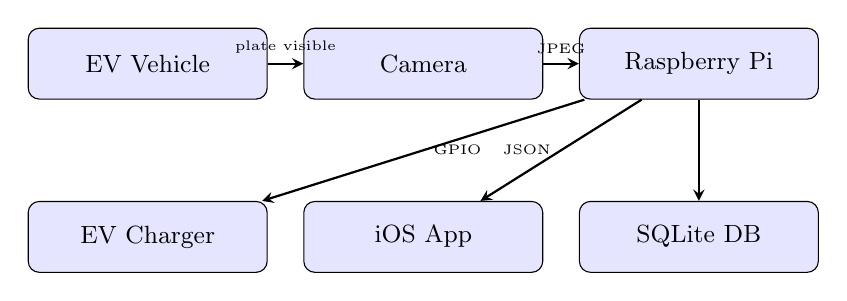
\begin{tikzpicture}[node distance=2.2cm, auto,
    block/.style={rectangle, draw, fill=blue!10, text width=2.8cm, text centered, rounded corners, minimum height=0.9cm, font=\small},
    cloud/.style={ellipse, draw, fill=orange!10, text width=2.2cm, text centered, minimum height=0.8cm, font=\small},
    arrow/.style={thick,->,>=stealth}]
    \node [block] (ev) {EV Vehicle};
    \node [block, right of=ev, node distance=3.5cm] (cam) {Camera};
    \node [block, right of=cam, node distance=3.5cm] (pi) {Raspberry Pi};
    \node [block, below of=pi] (db) {SQLite DB};
    \node [block, below of=cam] (ios) {iOS App};
    \node [block, below of=ev] (charger) {EV Charger};
    \draw [arrow] (ev) -- node[above]{\tiny plate visible} (cam);
    \draw [arrow] (cam) -- node[above]{\tiny JPEG} (pi);
    \draw [arrow] (pi) -- (db);
    \draw [arrow] (pi) -- node[left]{\tiny JSON} (ios);
    \draw [arrow] (pi) -- node[right]{\tiny GPIO} (charger);
\end{tikzpicture}
\caption{Product Context Diagram}
\label{fig:product_context}
\end{figure}

\subsection{Product Functions}
\begin{itemize}
    \item \textbf{Real-Time License Plate Detection:} YOLOv11 detects plates in live camera frames with sub-second latency.
    \item \textbf{OCR-Based Text Extraction:} EasyOCR extracts characters from cropped plate regions.
    \item \textbf{Pattern Validation:} Regex validator confirms standard plate formats.
    \item \textbf{Database Verification:} SQLite lookup retrieves owner information and account balance.
    \item \textbf{Authorization Signal:} JSON verification payload triggers the iOS app's success screen.
    \item \textbf{Live Visual Feedback:} Bounding boxes and OCR text overlaid on the iOS camera preview.
\end{itemize}

\subsection{User Classes and Characteristics}
\begin{itemize}
    \item \textbf{EV Drivers:} End users who benefit from app-free charging. Zero technical knowledge required.
    \item \textbf{Station Operators:} Personnel who deploy and configure the system, requiring basic Linux/networking skills.
    \item \textbf{System Administrators:} Technicians who maintain the database and update the model.
\end{itemize}

\subsection{Technological Stack}
\begin{table}[H]
\centering
\caption{Technology Stack}
\renewcommand{\arraystretch}{1.3}
\begin{tabular}{|l|l|}
\hline
\textbf{Component} & \textbf{Technology} \\
\hline
Edge Hardware & Raspberry Pi 4B (ARM Cortex-A72, 4\,GB RAM) \\
\hline
Server Language & Python 3.9+ \\
\hline
Client Language & Swift 5.9 \\
\hline
Inference Runtime & ONNX Runtime (aarch64) \\
\hline
Object Detection & YOLOv11 (INT8 Quantized) \\
\hline
OCR Engine & EasyOCR \\
\hline
Communication & WebSocket (asyncio) \\
\hline
Database & SQLite 3 \\
\hline
iOS Frameworks & SwiftUI, AVFoundation, Combine \\
\hline
Image Processing & OpenCV \\
\hline
Version Control & Git \& GitHub \\
\hline
\end{tabular}
\end{table}

\subsection{Operating Environment}
The system operates across two primary environments:
\begin{itemize}
    \item \textbf{Edge Server Environment:} Raspberry Pi 4B running Raspberry Pi OS (64-bit Debian-based Linux). The Python server runs as a systemd service, starting automatically on boot.
    \item \textbf{iOS Client Environment:} iPhone running iOS 16+ with camera permissions granted. The app connects to the Pi over the local network via WebSocket.
\end{itemize}

\subsection{General Constraints}
\begin{itemize}
    \item Processing speed is limited by the Raspberry Pi's ARM CPU (no GPU acceleration).
    \item Camera quality and lighting conditions affect detection accuracy.
    \item OCR accuracy degrades on damaged, dirty, or non-standard plates.
    \item The system requires both the Pi and camera to be on the same local network.
\end{itemize}

\subsection{Design \& Implementation Constraints}
\begin{itemize}
    \item The system shall fit within the Raspberry Pi's 4\,GB RAM constraint.
    \item The WebSocket protocol must handle binary image data efficiently.
    \item The iOS application must handle camera permissions and background session management.
    \item The ONNX model must use only operators supported by the ARM CPU execution provider.
    \item All \texttt{ConvInteger} nodes must use UINT8 weights (ARM NEON limitation).
\end{itemize}

\subsection{Assumptions and Dependencies}
\subsubsection{Assumptions}
\begin{itemize}
    \item Adequate lighting is available at the charging bay for plate visibility.
    \item License plates follow a standard Indian alphanumeric format (e.g., KL07AB1234).
    \item The Raspberry Pi has local network connectivity for WebSocket communication.
    \item Vehicles park within 2--5 meters of the camera, providing sufficient plate resolution.
\end{itemize}

\subsubsection{Dependencies}
\begin{itemize}
    \item ONNX Runtime for ARM (\texttt{aarch64}) must support the patched UINT8 \texttt{ConvInteger} operator.
    \item EasyOCR requires PyTorch and pre-trained English language models.
    \item The iOS application requires iOS 16+ and camera permissions.
    \item SQLite3 is included in the Python standard library.
\end{itemize}

\section{External Interface Requirements}
\subsection{User Interfaces}
The system presents two user interfaces:
\begin{itemize}
    \item \textbf{iOS Application:} A native SwiftUI interface showing the live camera preview, real-time bounding box overlays with OCR text, connection status indicator, and a verification success modal displaying the vehicle owner's name and account balance.
    \item \textbf{Server Console:} A terminal-based logging interface displaying OCR results, regex validation status, database lookup outcomes, and verification signals.
\end{itemize}

\subsection{Hardware Interfaces}
\begin{itemize}
    \item \textbf{Camera Module:} CSI camera or iOS device camera for frame capture.
    \item \textbf{Raspberry Pi 4B:} Edge computing unit for inference.
    \item \textbf{GPIO Relay (Future):} For triggering the physical charger upon authorization.
    \item \textbf{Network Interface:} Wi-Fi or Ethernet for WebSocket communication.
\end{itemize}

\subsection{Software Interfaces}
\begin{itemize}
    \item \textbf{WebSocket Server:} Accepts binary JPEG frames, returns JSON detection/verification payloads.
    \item \textbf{ONNX Runtime:} Executes the quantized YOLOv11 model graph.
    \item \textbf{EasyOCR:} Extracts text from cropped plate regions.
    \item \textbf{SQLite:} Stores and retrieves vehicle records via Python's \texttt{sqlite3} module.
\end{itemize}

\subsection{Communication Interface}
\textbf{Network Communication:} WebSocket protocol over TCP/IP for bidirectional, low-latency communication. Messages are binary (client $\to$ server: JPEG frames) and text (server $\to$ client: JSON payloads).

\section{Hardware \& Software Requirements}
\subsection{Hardware Requirements}
\begin{table}[H]
\centering
\caption{Hardware Requirements}
\renewcommand{\arraystretch}{1.3}
\begin{tabular}{|l|l|}
\hline
\textbf{Component} & \textbf{Specification} \\
\hline
Edge Computer & Raspberry Pi 4B, 4\,GB RAM \\
\hline
Camera & CSI or USB, minimum 2\,MP \\
\hline
iOS Device & iPhone SE 2nd gen or newer \\
\hline
Storage & MicroSD 16\,GB minimum \\
\hline
Network & Wi-Fi or Ethernet \\
\hline
Power Supply & 5V/3A USB-C for Pi \\
\hline
\end{tabular}
\end{table}

\subsection{Software Requirements}
\begin{table}[H]
\centering
\caption{Software Requirements}
\renewcommand{\arraystretch}{1.3}
\begin{tabular}{|l|l|}
\hline
\textbf{Component} & \textbf{Version / Details} \\
\hline
Raspberry Pi OS & 64-bit (Bookworm) \\
\hline
Python & 3.9+ \\
\hline
ONNX Runtime & 1.16+ (aarch64) \\
\hline
OpenCV & opencv-python-headless 4.x \\
\hline
EasyOCR & 1.7+ \\
\hline
websockets & 12.0+ \\
\hline
Xcode & 15+ \\
\hline
iOS & 16+ \\
\hline
SQLite & 3.x (built-in) \\
\hline
\end{tabular}
\end{table}

\section{Functional Requirements}
The system shall:
\begin{enumerate}
    \item Accept live video frames via WebSocket connection from a camera client.
    \item Decode incoming JPEG binary data into BGR image arrays using OpenCV.
    \item Preprocess images to 640$\times$640 pixels with normalization for YOLO input.
    \item Detect license plates using the quantized YOLOv11 INT8 model via ONNX Runtime.
    \item Apply Non-Maximum Suppression (NMS) to filter overlapping detections.
    \item Crop detected plate regions from the original image.
    \item Extract text from cropped plates using EasyOCR.
    \item Clean OCR output by removing whitespace and converting to uppercase.
    \item Validate cleaned text against configurable regex patterns.
    \item Query the SQLite database with validated plate strings.
    \item Generate and send a JSON verification response upon successful database match.
    \item Send JSON detection coordinates for bounding box rendering when no verification occurs.
    \item Stop sending frames and display a success modal on the iOS client upon verification.
\end{enumerate}

\section{Non-Functional Requirements}
\subsection{Performance Requirements}
\begin{itemize}
    \item End-to-end pipeline latency shall be under 1 second on the Raspberry Pi.
    \item The system shall process frames at a minimum of 2 FPS.
    \item The iOS application shall maintain 30 FPS camera preview with overlay rendering.
    \item SQLite queries shall complete within 1\,ms for the expected database size ($<$100,000 records).
\end{itemize}

\subsection{Security Requirements}
\begin{itemize}
    \item Plate images shall be processed locally and never transmitted to external cloud servers.
    \item Only the verification result (owner name, balance) shall be transmitted over the network.
    \item Database access shall be restricted to the local edge node.
    \item WebSocket connections should use WSS (TLS-encrypted) in production deployments.
\end{itemize}

\subsection{Safety Requirements}
\begin{itemize}
    \item The system shall not authorize charging for unregistered vehicles.
    \item The system shall not authorize charging for vehicles with insufficient balance.
    \item False positive rate for plate detection must be below 1\%.
\end{itemize}

\subsection{Software Quality Requirements}
\begin{itemize}
    \item \textbf{Reliability:} Consistent detection accuracy across varying lighting conditions.
    \item \textbf{Usability:} Zero training required for end users (EV drivers).
    \item \textbf{Scalability:} Each charging bay operates as an independent edge node.
    \item \textbf{Maintainability:} Modular architecture allows independent updates to model, OCR, or database.
    \item \textbf{Portability:} The Python server runs on any Linux-based ARM SBC.
\end{itemize}
